\clearpage\section{Method \& Materials}
We start a basic description and simulation of the measurement setup. Subsequently, the basic characterization of a quartz crystal is researched and we proceed to experiment with its amplitude-frequency dependence. Afterwards, the crystal is coated, and the behavior of the system with the introduction of different chemical compounds is investigated. 

\subsection{Experimental set-up}
The set-up consists of the electrical system to drive the crystals and measure its response, and of the system to bring the coated crystals in contact with gasses. The two systems will be described consecutively in the following sections.

\subsubsection{Electrical system}
A basic overview of the electrical system is shown in \autoref{fig:oveele}. The signal of a lock-in amplifier is amplified and buffered before exciting the crystal. The current is probed and this signal is fed back into the lock-in amplifier to measure the response of the crystal. The current flowing through the crystal is indicative of the impedance of the crystal, and thus whether the crystal is in resonance. For a detailed schematic and an overview of all used components, see \autoref{AP:schematic}

\begin{figure}
	\centering
		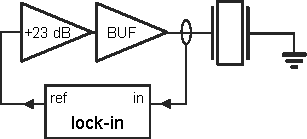
\includegraphics[width=\textwidth]{figures/oveele.pdf}
	\caption{Schematic overview of the electrical system of the experimental set-up. }
	\label{fig:oveele}
\end{figure}

\subsection{Crystal analysis}
The goals of the first phase are to choose a resonator and find benchmark impedance-frequency data of the chosen resonator. 

Since a mechanical resonator is needed to react to the change of mass, but it is desirable to drive and analyze the system electronically, a piezoelectric resonator is used as a transformer between the electronic and mechanical signal. Piezoelectric devices exist with a Q-factor of up to XXX, but they are very expensive. Ceramic resonators are cheap, but they lack stability and have low Q-factors XXX. A good middle ground is a quartz crystal oscillator, since they have Q-factors up to $10^6$, and are readily available because of their use in almost any electronic device on the market. 

Quartz crystals come in a variety of fundamental frequencies, shapes and sizes. For this experiment a large crystal is preferred over a small crystal, since it eases polymer coating. The fundamental frequency is preferably small, since it loosens bandwidth requirements of all components in the circuit and reduces crosstalk and phase lag XXX. The most common crystal shapes are a planar shear resonator and a tuning fork. Since the tuning fork has an irregular shape, it is hard to get an even coating. The first tests resulted in a coating which filled up the gap XXX. 

The circuit used in the first test is 

\subsubsection{Measurement}
Since the crystal is driven by a voltage 

\subsection{Gas mixture set-up}
To measure the response of the coated quartz crystals to gasses, a setup is needed to put the quartz crystal inside a gas mixture. The most important parameters of the gas mixture are the homogeneity, the accuracy of the mixing ratio and the pressure. It is possible to make a gas mixing set-up, but gas mixtures specifically for gas sensor calibration are available on the market as well. The calibration mixtures would have a higher concentration accuracy, whereas the gas mixture setup would have a higher flexibility. When using off-the-shelve gas mixtures, a new pre-made gas mixture would have to be bought. Therefore a gas mixing set-up will be made. 